% Setup - do not change
\documentclass[11pt]{article}
\usepackage[top=0.9in, left=0.9in, bottom=0.9in, right=0.9in]{geometry} 
\usepackage{parskip}

\usepackage[english]{babel}
\usepackage[utf8]{inputenc}
\usepackage{amsmath,amsthm,amssymb,graphicx,pdfpages,lipsum,hyperref}
\usepackage[none]{hyphenat}
\usepackage{csquotes}

\setlength\parindent{0pt}
%%%%%%%%%%%%%%%%%%%%%%%%%%%%%%%%%%%%%%%%%%%%%%%%%%%%%%%%%%%%%%%%%%%
% add other packages here if required
\usepackage{enumitem}
\usepackage{textcomp}
\usepackage{booktabs}
\usepackage{placeins}
\usepackage{wrapfig}
\graphicspath{{../plots/}}

%% Bibliography are specified in this file. You can also choose inline bib style if you want to. But make sure your citation style is consistent (and proper)
% For more details on citation: https://library.unimelb.edu.au/recite
\usepackage[sorting = none]{biblatex}
\addbibresource{references.bib}

%%%%%%%%%%%%%%%%%%%%%%%%%%%%%%%%%%%%%%%%%%%%%%%%%%%%%%%%%%%%%%%%%%% the '%' symbol denotes comments

% Begin document creation
% DELETE THE \lipsum PLACEHOLDERS WHEN YOU BEGIN
\title{\textbf{Insert Title} \\ Insert Subtitle}
\author{
Insert Student Name \\
Student ID: XXXXXX \\
%% Replace the link with your github repo
% 1. Remember to escape underscore (\_) in the link.
% 2. Remember to include the commit you want to submit in the link
\href{INSERT GITHUB REPO HERE i.e https://github.com/MAST30034-Applied-Data-Science/mast30034\_p1\_template/tree/fd9f1dd17fdbcb5b119b70c93a22da8210d44fd7}{Github repo with commit}
}

\begin{document}
\maketitle

\section{Introduction}
% Link to a 30 min tutorial if you require revision: https://www.overleaf.com/learn/latex/Learn_LaTeX_in_30_minutes

\LaTeX{} has many caveats, you should search stack overflow for latex tips whenever you feel something looks bad, for instance:
When `` quoting '', should be used instead of ". For example, ``test'' vs "test".

% use \textbf{} for bold text and \textit{} for italic. 
% \texttt{} creates code blocks akin to `code ticks` in markdown
\textbf{Please refer to the spec, the word count and page count is strict.} Feel free to change the section headings (and we recommend you do).

Always remember to cite anything that is not your work. For instance, you must cite the datasets like this \cite{2022sensorreading, 2022sensorlocation}.
% Example here used biblatex to manage citations: https://www.overleaf.com/learn/latex/Bibliography_management_with_biblatex , You are free to choose your own way for managing references if biblatex seems too hard.

\lipsum[7]

% You can have \section{}, \subsection{}, and \subsubsection{}, \section*{}, \subsection*{}, and \subsubsection*{}
\section{Preprocessing}
The TLC receives trip records from the technology providers in each vehicle and makes no promise that they are accurate \cite{tlctripdata}, so every record is checked before use. All checks, cut-offs and removals are run on the full data in PySpark, one month at a time. Table~\ref{tab:cleaning} gives the shape of the data after each step, and the points below give the reason for each step.

\begin{table}[ht]
    \centering
    \small
    \caption{Shape of the taxi data after each cleaning step. \emph{Removed} is the share of raw rows removed by that step; -- marks a step that does not apply to the service.}
    \label{tab:cleaning}
    \begin{tabular}{@{}rl rrr rrr@{}}
        \toprule
        & & \multicolumn{3}{c}{Yellow taxi} & \multicolumn{3}{c}{HVFHV (Uber and Lyft)} \\
        \cmidrule(lr){3-5} \cmidrule(l){6-8}
        & Step & Rows & Cols & Removed & Rows & Cols & Removed \\
        \midrule
        & Raw files (Jan 2023--Dec 2025) & 128,202,548 & 19--20 & & 715,550,152 & 24--25 & \\
        1 & Keep used columns & 128,202,548 & 14 & 0\% & 715,550,152 & 10 & 0\% \\
        2 & Pickup in the file's month & 128,201,184 & 14 & $<$0.01\% & 715,550,152 & 10 & 0\% \\
        3 & Drop-off after pickup & 127,625,804 & 14 & 0.45\% & 715,519,470 & 10 & $<$0.01\% \\
        4 & Fare collected (payment type) & 124,407,631 & 14 & 2.51\% & -- & & \\
        5 & Positive fare & 123,959,890 & 14 & 0.35\% & -- & & \\
        6 & Known rate code & 122,483,608 & 14 & 1.15\% & -- & & \\
        7 & Positive driver pay & -- & & & 714,346,062 & 10 & 0.16\% \\
        8 & Outlier caps & 121,460,780 & 14 & 0.80\% & 714,221,778 & 10 & 0.02\% \\
        9 & Trip group known & 120,568,974 & 14 & 0.70\% & 694,437,031 & 10 & 2.77\% \\
        \midrule
        & Cleaned (share of raw rows kept) & \multicolumn{3}{l}{120,568,974~$\times$~14 (94.0\%)} & \multicolumn{3}{l}{694,437,031~$\times$~10 (97.0\%)} \\
        \bottomrule
    \end{tabular}
\end{table}
\FloatBarrier % print Table 1 before the step bullets that refer to it

\subsection{Taxi trip data}
\begin{itemize}[leftmargin=*, itemsep=1pt, topsep=2pt]
    \item \textbf{One schema (step 1).} Column types and names change during 2023, so each month is cast to one schema before stacking, keeping only the columns used later. The extra raw column in 2025 records the new toll fee.
    \item \textbf{Nulls are kept.} Yellow nulls fall in four columns only, and in every month on exactly the Flex Fare trips (payment type 0, a price agreed upfront \cite{tlcyellowdict}). These are real trips that grew from 3.4\% of yellow rows in 2023 to 23.8\% in 2025, so dropping them would fake a fall in trips after the toll. None of the four columns is used, so nothing is imputed. The toll fee column is null only before the toll began.
    \item \textbf{Impossible times (steps 2--3).} A pickup outside the file's month has a wrong date, and a drop-off at or before pickup gives no trip length. 93\% of the yellow rows removed at step 3 come from vendor 7 (Helix), new in December 2024 \cite{tlcyellowdict}, which records this on every trip. Its pickups are in the tolled area as often as yellow pickups overall (56.4\% and 56.8\%), so removing it does not favour either side of the comparison.
    \item \textbf{Unreliable fares (steps 4--6, yellow).} Payment types 3, 4 and 6 are no charge, dispute and voided trips, and rate code 99 is unknown \cite{tlcyellowdict}, so their revenue cannot be trusted. Most negative fares are reversals: 88--92\% of negative cash, no-charge and dispute fares cancel another row exactly, and keeping both rows would count the trip twice. A zero fare is below the \$3.00 initial charge every metered trip records \cite{tlcfare}, so it is not a correct reading either. Flex Fare trips skip steps 5--6, because their negative fares (20.5\% of Vendor 2's in 2025) cancel nothing. They are kept with unknown revenue, which with the unmeasured trips below leaves 2025 yellow earnings known for 92.1--94.8\% of trips in each zone group, against 98\% or more in 2023--2024.
    \item \textbf{Unpaid trips (step 7, HVFHV).} Driver pay is what the driver earns after commission, excluding tips \cite{tlchvfhvdict}. It is the Uber and Lyft earnings outcome, so zero or negative pay is removed. Most of these rows are from January--March 2023, before the comparison period.
    \item \textbf{Outliers (step 8).} The caps remove trips under 1 minute or over 5 hours, over 100 miles, over 60 mph on average, or paying over \$500. They were set from full-data histograms where each tail turns into impossible values, and sit well above every 99.9th percentile (under 2 hours, 54 miles, 48 mph and \$152). A distance of 0 is not an outlier but an unmeasured trip: the trip still happened, so it is kept and counted, with its earnings set to unknown like the Flex Fare trips above.
    \item \textbf{Unknown ends (step 9).} Zones 264 (``Unknown'') and 265 (``Outside of NYC'') have no shape \cite{tlczones}. A trip with one end in them is still kept when its other end is in the tolled area, because that end alone makes it treated, whichever place the unknown end stands for. It is removed only when the known end is a ring or control zone, because that end alone cannot say whether the trip touched the tolled area. No treated trip is therefore removed here, and the rule takes 2.4\% of 2025 HVFHV ring rows (0.4\% of yellow).
    \item \textbf{Summary table.} Earnings are driver pay, or for yellow the fare plus the driver's own surcharges, after removing the city and MTA charges that Vendor 1 adds to the same column. \emph{Earnings per engaged hour} divides that by the time from pickup to drop-off. It is left unknown for a shared HVFHV ride, whose driving hour is split with another trip, and for the unmeasured trips above; together those are 1.1 to 1.9\% of HVFHV trips in each group and period, so the measure is known for at least 98\% of them throughout. Trips are summed per service $\times$ pickup zone $\times$ drop-off zone group $\times$ date $\times$ time band, with medians taken over every trip and empty combinations kept as 0 trips. The result is 11,880,640~$\times$~14: 2 services $\times$ 1,355 zone pairs $\times$ 1,096 days $\times$ 4 bands. A pair is one of the 263 pickup zones with one of the 5 drop-off groups, plus 40 cells for the unknown ends step 9 keeps (the 38 tolled zones with an unknown drop-off, and zones 264 and 265 with a tolled drop-off). It counts all 815 million cleaned trips in a table small enough to model, and its totals are checked against Table~\ref{tab:cleaning}.
\end{itemize}

\subsection{External data}
\begin{itemize}[leftmargin=*, itemsep=1pt, topsep=2pt]
    \item \textbf{Zone groups.} The MTA list of tolled zones (38~$\times$~2) \cite{mtacbdzones} is joined to the TLC zone lookup (265~$\times$~4) on zone ID, with each zone's distance to the tolled area from the TLC shapefile (263~$\times$~7) \cite{tlczones}: 265~$\times$~8. Zones within 1 km form a \emph{ring} (19 zones, 13 across a river), since riders can walk out of the tolled area and drivers can wait at its edge; as controls they would overstate the toll's effect. Any cut-off from 0.94 to 1.05 km gives the same ring. The other 206 zones are controls. A trip is \emph{treated} if either end is in the tolled area, otherwise \emph{ring} if either end is in the ring.
    \item \textbf{Weather and holidays.} NOAA daily Central Park records \cite{noaaghcnd}, 1,096~$\times$~7, already metric. The station ID is dropped and the one missing snow depth (17 September 2025, 21\textdegree C) is set to 0: 1,096~$\times$~6. A flag marks the US federal holidays of 2023--2025 \cite{opmholidays}: 35 dates, because the two that fell at a weekend are flagged on the observed weekday as well.
    \item \textbf{Joins.} Both join on date: 11,880,640~$\times$~14 $\to$ $\times$~19 $\to$ $\times$~20, with the row count checked unchanged. Both models are fitted to this table.
\end{itemize}

\textbf{Does cleaning bias the comparison?} A rule can bias it if it removes a larger share from one group after the toll. From 2024 to 2025 the share of yellow rows removed rose by 1.6 points for treated trips and 1.8 for control trips, a gap of at most 0.2 points. For HVFHV the shares are flat: no treated row is removed for an unknown end, and the only rule that treats the groups differently takes 2.18\% of ring rows in 2024 against 2.38\% in 2025, a gap of 0.2 points on trips that are neither treated nor control. Cleaning therefore cannot account for more than a fraction of a point of the treated-versus-control gaps below.

\section{Analysis and Geospatial Visualisation}
\label{sec:analysis}
Every before-and-after comparison below sets the toll period, 5 January to 31 December 2025, against the same dates of 2024, so both windows hold the same seasons and the four pre-toll days of January 2025 are left out. Percentages are changes between those two windows unless stated otherwise.

\subsection{Distributions, missing values and outliers}
Trip length, distance, speed, fare or driver pay, and earnings per engaged hour were binned over every raw row and again over every cleaned trip, on the full data rather than a sample. Table~\ref{tab:distributions} reads the quantiles of the first four off those bins.

\begin{table}[ht]
    \centering
    \small
    \caption{Each attribute over every raw row with a positive trip time and distance, read off full-data histograms with fine bins (0.1 minute, 0.05 mile, 0.1 mph, \$0.25). The cut-off is the outlier rule of Table~\ref{tab:cleaning}, step 8.}
    \label{tab:distributions}
    \begin{tabular}{@{}l rrrr rrrr@{}}
        \toprule
        & \multicolumn{4}{c}{Yellow taxi} & \multicolumn{4}{c}{HVFHV (Uber and Lyft)} \\
        \cmidrule(lr){2-5} \cmidrule(l){6-9}
        Attribute & Median & IQR & 99.9th & Cut-off & Median & IQR & 99.9th & Cut-off \\
        \midrule
        Trip length (min) & 13.2 & 8.1--21.3 & 119.3 & 1--300 & 16.2 & 10.1--25.7 & 107.4 & 1--300 \\
        Trip distance (mi) & 1.85 & 1.10--3.60 & 30.2 & 100 & 3.05 & 1.60--6.35 & 53.5 & 100 \\
        Average speed (mph) & 9.5 & 7.1--13.2 & 47.8 & 60 & 11.6 & 8.8--16.6 & 47.2 & 60 \\
        Fare or driver pay (\$) & 13.75 & 9.50--22.75 & 141.75 & 500 & 15.25 & 9.00--25.50 & 151.5 & 500 \\
        \bottomrule
    \end{tabular}
\end{table}

\begin{itemize}[leftmargin=*, itemsep=1pt, topsep=2pt]
    \item \textbf{All five are right skewed.} In Table~\ref{tab:distributions} the upper quartile is 1.4 to 2 times the median while the 99.9th percentile is 4 to 17 times it, and earnings per engaged hour (\S2.1) behaves the same way, so every earnings figure below is a median. The typical trip is short and cheap, 13.2 minutes and \$13.75 of fare for yellow and 16.2 minutes and \$15.25 of driver pay for HVFHV, which is worth holding on to under the percentages below.
    \item \textbf{Cleaning cuts the tails and leaves the body alone.} Each curve peaks in the same bin before and after, and below about 100 minutes the two trip-length curves lie on top of each other. What goes is the pile in the end bins: 0.49\% of raw yellow rows sit under $-$\$95 an hour and 0.94\% at \$395 or more, against 0.01\% and 0.12\% after. The cut-offs are deliberately loose, each at least twice the matching 99.9th percentile in Table~\ref{tab:distributions}, so they remove impossible readings rather than unusually busy trips. HVFHV has almost no tail to cut, 0.021\% of raw rows at \$395 an hour or more against 0.017\% of cleaned trips, because those trips break no other rule. Piles this small cannot move a median.
    \item \textbf{Nothing in the taxi data is imputed.} Nulls fall in four yellow columns only and always on Flex Fare trips, and none of the four is used here, so the trips are kept and counted with nothing filled in. The one missing NOAA snow depth is set to 0.
    \item \textbf{The nulls carry a finding.} Flex Fare grew from 3.4\% of yellow rows in 2023 to 23.8\% in 2025 and grew unevenly, 4.1\% to 38.1\% of control trips against 3.5\% to 24.4\% of treated trips, so the yellow control group changed over the window for a reason the toll did not cause: HVFHV carries the argument below and yellow is read as a check on it.
\end{itemize}

\subsection{Trips touching the zone lost ground to the rest of the city}
Figure~\ref{fig:relative} divides each month's treated (and ring) trips by the same month's control trips, indexed so each service's 2024 average is 100. Seasons, holidays and citywide shocks hit all three groups and mostly cancel in the ratio, so a line falling after the toll marks a group losing trips to the rest of the city.

\begin{figure}[htb]
    \centering
    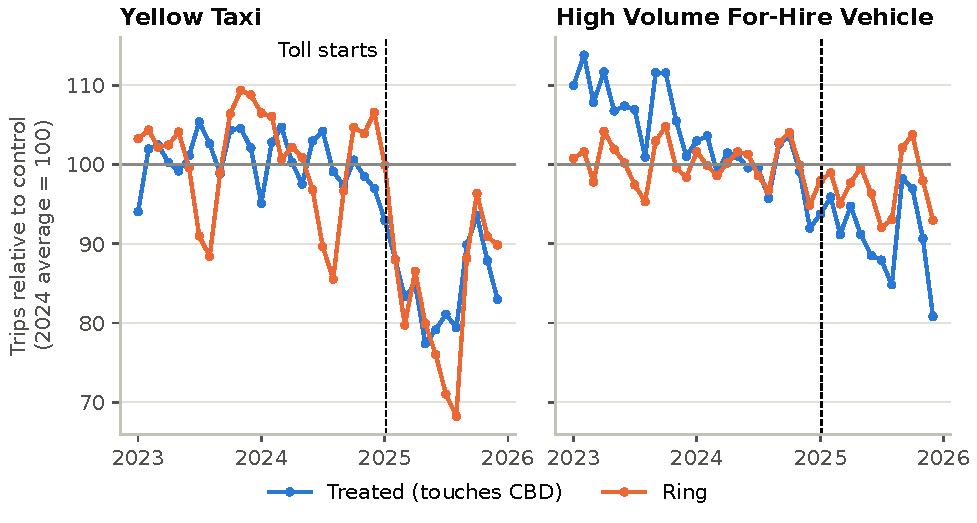
\includegraphics[width=\textwidth]{fig1_relative_trips.pdf}
    \caption{Monthly trips touching the tolled zone, and trips touching the ring, each divided by that month's control trips and indexed to the service's 2024 average. The dashed line is 5 January 2025.}
    \label{fig:relative}
\end{figure}

From Figure~\ref{fig:relative} we see HVFHV treated trips averaging 91.9 against control in 2025, down from 100 in 2024, while ring trips barely moved (97.3). About 227,000 HVFHV trips a day touched the zone before the toll and about 219,000 after. So the toll cost drivers trips inside the zone, and those trips did not reappear at its edge: ring trips adjacent to the zone were flat ($+0.1\%$) and ring trips across the water rose 2.7\%, both below the $+5.4\%$ of the far control zones. But the treated line was already sliding before the toll, from 107.9 in 2023, so part of the fall is a trend the toll did not cause and Section~\ref{sec:modelling} has to test that before the gap can be read as an effect. Yellow looks worse and on inspection is not: yellow treated trips \emph{grew} 14.1\%, and the ratio fell only because yellow control trips grew far faster ($+56.6\%$ far, $+17.7\%$ near), in step with the uneven Flex Fare growth of \S3.1. A toll on entering Manhattan cannot plausibly add half again to yellow trips in the outer boroughs, so it is the denominator moving, not the numerator, and every yellow reading below is the same argument again.

The HVFHV line is unsteady within 2025 too, recovering to 99 in September and 98 in October before falling to 82 in December. Most of that swing is ordinary. December is the low month of the ratio in every year of the window (101.6 in 2023, 92.6 in 2024, 82.1 in 2025), and the October-to-December fall is of a familiar size: 10.0 points in 2023, 11.3 in 2024 and 15.8 in 2025. What is left is in the denominator. December 2025 control trips ran 9.4\% above December 2024, the fastest growth of any month in the toll period, while treated trips were 3.0\% down, a smaller fall than June ($-8.0\%$) or August ($-6.4\%$). So the December point is a seasonal low read over a fast-growing control group rather than a fresh loss inside the zone, and the event study in Section~\ref{sec:modelling}, which compares each month with the same month a year earlier, is where it is settled.

\subsection{Where the trips were lost, and what happened to earnings}
Figure~\ref{fig:zones} maps each pickup zone's change in HVFHV pickups. Zones averaging fewer than 10 pickups a day in 2024 are greyed out: at that rate the window holds about 3,600 trips, where chance alone moves a count by roughly 2\%. 256 of 263 zones clear the bar for HVFHV but only 114 for yellow, a second reason the yellow maps stay in the notebook.

\begin{figure}[htb]
    \centering
    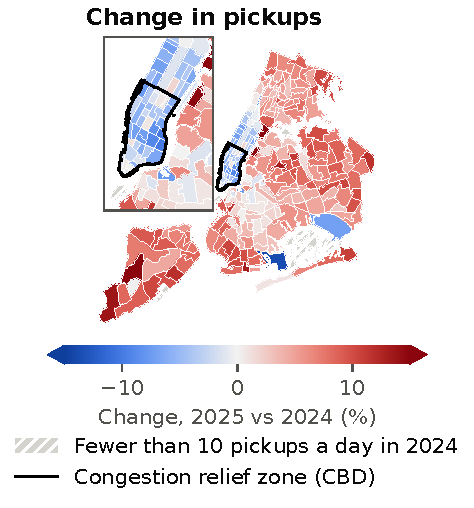
\includegraphics[width=0.5\textwidth]{fig2_zone_map.pdf}
    \caption{Change in HVFHV pickups by pickup zone, toll period against the same dates of 2024. The inset enlarges Manhattan and the outlined tolled zone.}
    \label{fig:zones}
\end{figure}

From Figure~\ref{fig:zones} we see pickups falling in almost every zone inside the cordon (median zone $-4.3\%$) and in the Manhattan zones immediately north of it ($-3.8\%$), while growing across most of the outer boroughs ($+5.9\%$). Apart from two thinly used outer-borough zones and the Brooklyn Navy Yard, the ten largest falls are all inside the zone and mostly residential: Alphabet City ($-10.1\%$), Stuy Town/Peter Cooper Village ($-10.0\%$), the East Village ($-9.0\%$) and Gramercy ($-8.2\%$). So the rides drivers lost started where people live inside the zone rather than at its offices and transport hubs, perhaps because those trips are short: on a short fare the flat \$1.50 charge is a larger share of the price, and it is also the trip a rider can most easily walk or take the subway instead. Trip length by zone was not measured here, so this reads the map rather than settles it, and it is the first thing worth measuring next.

\begin{wrapfigure}[20]{l}{0.47\textwidth}
    \vspace{-0.9\baselineskip}
    \centering
    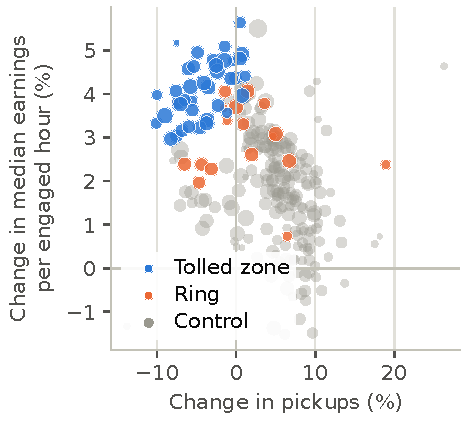
\includegraphics[width=0.45\textwidth]{fig3_zone_scatter.pdf}
    \caption{Each zone's two changes on one pair of axes, for the 256 zones of Figure~\ref{fig:zones}. Marker area grows with the zone's 2024 pickups.}
    \label{fig:scatter}
    \vspace{-1.2\baselineskip}
\end{wrapfigure}

Earnings ran the other way. Figure~\ref{fig:scatter} puts each zone's change in pickups against its change in median earnings per engaged hour, the medians taken over every trip rather than over the summary table's cell medians. Every one of the 38 zones inside the cordon gained, by 3.0 to 5.6\% an hour against 1.7\% in the median far control zone, and 33 of the 38 lost pickups while doing it. Across all 256 zones the two changes pull against each other (Spearman $\rho = -0.56$) and the cordon sits alone in the top left corner of the figure: fewer rides, better paid rides. On the 2024 base of \$54.65 an hour in the median cordon zone, the median gain of 4.1\% is about \$2.20 an hour, and the East Village went from \$54.20 to \$56.10. Inside the cordon, though, the gain does not follow the loss: the zones that lost most, Alphabet City ($-10.1\%$) and Gramercy ($-8.2\%$), gained 3.3 and 3.0\% an hour, \emph{less} than Midtown Center ($+0.7\%$ pickups, $+4.9\%$ an hour) or the World Trade Center ($+0.5\%$ and $+5.6\%$), so within the zone the two run mildly together ($\rho = +0.50$). A gain spread that evenly points to something acting on every trip in the zone rather than to thinner demand lifting the fares of the zones that emptied. The candidate is on the road, and the trips themselves can test it. Across all 464 million HVFHV trips picked up in the three groups, the median trip from a tolled zone ran 2.1\% faster after the toll (10.01 to 10.23 mph) and covered 2.9\% more ground in the same 18.3 minutes (2.80 to 2.88 miles), while control pickups went 1.4\% slower over 2.7\% less ground and ring pickups barely moved ($-0.2\%$ and $-1.3\%$). An engaged hour inside the zone therefore buys more distance, and distance is what the fare pays for. MTA speed data \cite{mtacbdspeeds}, which times every vehicle rather than only those carrying a passenger, agrees over its own window: 3.1\% faster inside the zone (8.74 to 9.01 mph) against $-1.1\%$ next to it and $-0.9\%$ for the rest of the city.

Two zones moved against their neighbours: Randalls Island ($+26.3\%$), a park and event venue with almost no residents, and Queensbridge/Ravenswood ($+18.9\%$), a ring zone one bridge from Midtown. A ring zone taking a fifth more pickups while the zone across the river loses them is the most directly usable finding here, and Section~\ref{sec:recommendations} returns to it.

\subsection{When the trips were lost}
Figure~\ref{fig:bandday} asks when. Panel (a) gives the change in treated trips for each time band and day of week; panel (b) divides that by the change in control trips, $(1 + \text{treated change})/(1 + \text{control change}) - 1$, so $-8$ means treated trips ended up 8\% below where the control group's change alone would have put them. It is a raw version of the model in Section~\ref{sec:modelling}, without weather or other controls.

\begin{figure}[htb]
    \centering
    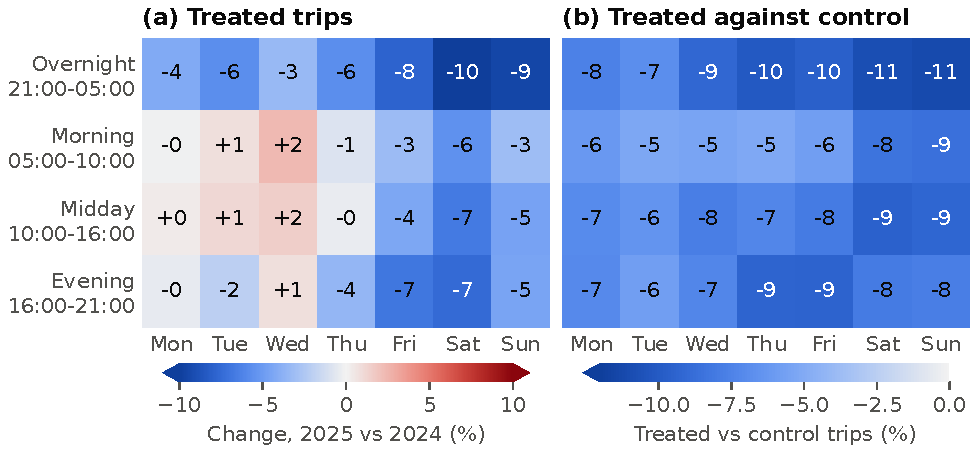
\includegraphics[width=\textwidth]{fig4_band_day.pdf}
    \caption{Change in HVFHV trips touching the tolled zone by time band and day of week, toll period against the same dates of 2024: on their own (a) and relative to control trips (b). Every cell of (b) is negative, so it uses a one-sided scale.}
    \label{fig:bandday}
\end{figure}

From Figure~\ref{fig:bandday}(b) we see HVFHV treated trips falling against control in all 28 cells, by 5 to 11\%, which is worth stating on its own: the loss is not confined to a rush hour or to weekdays. The gap is widest overnight ($-7$ to $-11\%$) and at weekends ($-8$ to $-11\%$ outside the evening), narrowest on weekday mornings ($-5$ to $-6\%$). Panel (a) says where that comes from: treated trips on Monday to Thursday mornings and middays hardly moved ($-1$ to $+2\%$), while overnight and weekend treated trips fell 3 to 10\%. So what the toll removed looks like discretionary travel rather than commuting, probably because a rider due at work at 8am has to be in the zone and a rider going out at midnight does not, and because \$1.50 is a larger share of a cheap off-peak fare than of a busy peak one. That gives Section~\ref{sec:modelling} a testable steer: a time-band model should find its largest effect overnight, and if it does not, weather or the mix of days is doing more than this raw comparison admits. Yellow repeats the shape at larger sizes ($-8$ to $-35\%$), and again on control growth (18 to 89\% by cell) rather than a treated fall, so its panels stay in the notebook.

\subsection{What the trip counts cannot show}
One measure cuts against the story. The wait from ride request to pickup got slightly shorter inside the zone and longer outside it: averaged over each year's monthly medians it went from 3.80 to 3.76 minutes for treated trips and from 4.09 to 4.20 for control trips, with the 90th percentile moving further (8.12 to 7.99 against 7.98 to 8.58). Shorter waits alongside fewer trips point to more idle drivers per rider inside the zone. So a driver working the zone may be taking fewer rides per hour online even as each engaged hour pays better, and the trip records cannot settle it, because a driver cruising empty for twenty minutes leaves no row in them. This is the one question the exploration raises that the data cannot answer, and it bounds what the earnings results in Section~\ref{sec:modelling} may claim.

\section{Modelling}
\label{sec:modelling}
Example of a maths equation:
\begin{equation}
    Y = X\beta + \epsilon
\end{equation}

Example of an aligned equation (\& denotes the symbol to align):
\begin{align*}
    E[\mathbf{y}] &= X\beta + E[0] \\
                  &= X\beta
\end{align*}

Example of an in-line equation $\epsilon \sim N(0, 1)$ \\

\section{Discussion}
\lipsum[9]

\section{Recommendations}
\label{sec:recommendations}
\lipsum[10]

\section{Conclusion}
\lipsum[14]


\clearpage

% BEGIN REFERENCES SECTION
\printbibliography

\end{document}